\documentclass[a4paper,12pt]{article}

% Packages
\usepackage{float}
\usepackage{xcolor}
\usepackage[utf8]{inputenc}
\usepackage{fancyhdr}
\usepackage[left = 0.6 in, right = 0.6 in, top = 1 in, bottom = 1 in, headsep = 0.5 in]{geometry}
\usepackage[normalem]{ulem}
\usepackage{enumerate}
\usepackage{pgfplots}
\usepackage{titling}
\pgfplotsset{width=8cm,compat=1.9}
\usepackage{stackengine}
%\pagenumbering{gobble}
\usepackage[fleqn]{amsmath}
\usepackage{amssymb}
\usepackage[T1]{fontenc}
\usepackage{fancybox}
\usepackage{longtable}

\hfuzz = 100pt

%%% Horizontal Line Command
\makeatletter
  \newcommand*\variableheghtrulefill[1][.4\p@]{%
    \leavevmode
    \leaders \hrule \@height #1\relax \hfill
    \null
  }
\makeatother
%%%

%%% Header & Footer
\fancyhf{}
\renewcommand{\footrulewidth}{0.1mm}
\fancyhead[L]{Matteo Esposito, William Ngo, Spyros Orfanos}
%\fancyhead[C]{Assignment 1}
\fancyhead[R]{STAT 497-H}
%\fancyfoot[L]{ID: 40024121, 40025959, 400XXXXX}
%\fancyfoot[C]{Concordia University}
\fancyfoot[R]{\thepage}

\pagestyle{fancy}
%%%

% Code formatting
\def\code#1{\texttt{#1}}

\renewcommand\maketitlehooka{\null\mbox{}\vfill}
\renewcommand\maketitlehookd{\vfill\null}

% Custom settings
\setlength{\parskip}{0.75em}  % Paragraph spacing
\setcounter{section}{-1} % Page numbers to start on page 1
\setlength\parindent{0pt} % Remove indenting from entire file
\def\layersep{2.5cm}

\title{\textbf{Assignment 3}}
\author{STAT 497-H | Reinforcement Learning}
\date{Matteo Esposito (40024121), William Ngo (40031586), Spyros Orfanos (40032280)}

%%%%%%%%%%%%%%%%%%%%%%%%%%%%%%%%%%%%%%%%%%%%%%%%%%%%%%%%%%%%%%%%%%%%%%%%%%%%%%%%

\begin{document}
\begin{titlingpage}
  \maketitle
  \centering
  \vfill
  {\large{Concordia University}}\par
  {\large{April 14th, 2019}}
\end{titlingpage}

\newpage

\subsection*{Question 1}

\textbf{a)} Action-value function for policy $\pi$.

\begin{figure}[ht]
  \centering
    $\pi
    =
    \begin{bmatrix}
      \pi(1|1) = 0.7 & \pi(2|1) = 0.2 & \pi(3|1) = 0.1 \\
      \pi(1|2) = 0.1 & \pi(2|2) = 0.7 & \pi(3|2) = 0.2 \\
    \end{bmatrix}$       
  \end{figure}

\begin{figure}[ht]
  \centering
    $\code{PolicyAVF}
    =
    \begin{bmatrix}
      12.57745 & 12.10109 & 11.10109 \\
      11.05382 & 10.79200 & 11.10109
    \end{bmatrix}$       
\end{figure}

\textbf{b)}, \textbf{c)} See \code{main.R} code.

% Q: Among the three values tested for n, which seems to be the best
% for the current problem?

\textbf{d)} For the given problem, $n=20$ seems to be the best as its RMSE value decays
at a quicker rate compared to the $n=1$ and $n=5$ curves. 

\begin{figure}[H]
  \centering
  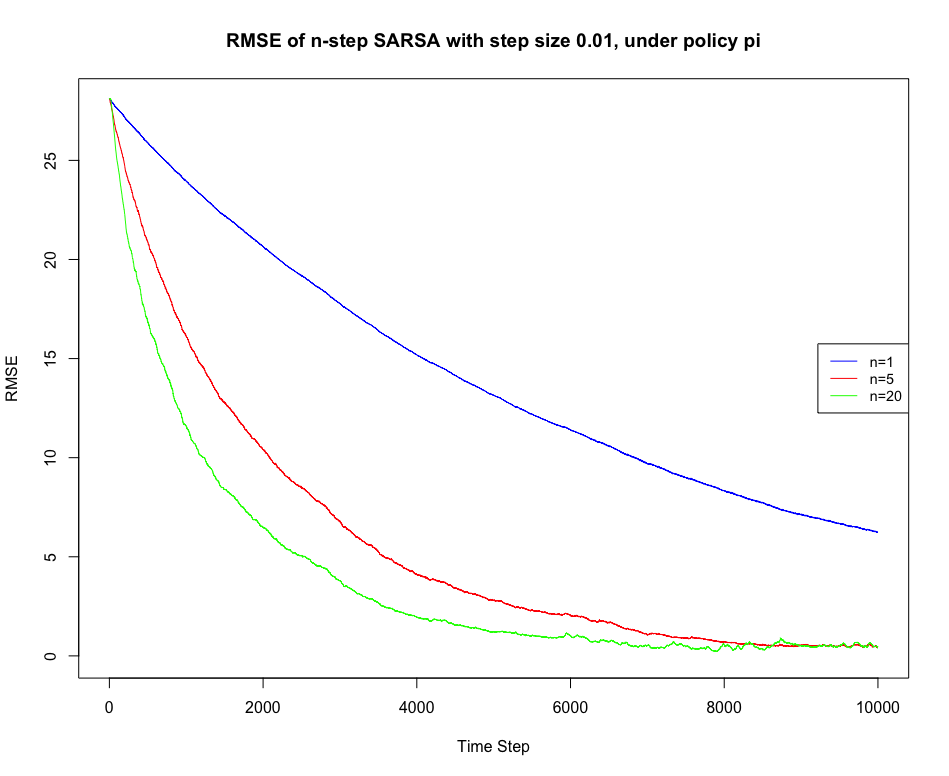
\includegraphics[width=14cm]{figures/1d.png}
\end{figure}

\textbf{e)} 

\begin{figure}[ht]
  \centering
    $\text{Estimated} = \hat{Q_{*}} =
    \begin{bmatrix}
      \hat{q_{*}}(1, 1) & \hat{q_{*}}(1, 2) & \hat{q_{*}}(1, 3) \\
      \hat{q_{*}}(2, 1) & \hat{q_{*}}(2, 2) & \hat{q_{*}}(2, 3)
    \end{bmatrix}   =  
    \begin{bmatrix}
      14.67647 & 14.18796 & 13.14585 \\
      13.10830 & 12.88070 & 13.19346
    \end{bmatrix}$      
\end{figure}

\begin{figure}[ht]
  \centering
    $\text{True} = Q_{*} =  
    \begin{bmatrix}
      {q_{*}}(1, 1) & {q_{*}}(1, 2) & {q_{*}}(1, 3) \\
      {q_{*}}(2, 1) & {q_{*}}(2, 2) & {q_{*}}(2, 3)
    \end{bmatrix}   =  
    \begin{bmatrix}
      14.70588 & 14.23529 & 13.23529 \\
      13.17647 & 12.91176 & 13.23529
    \end{bmatrix}$      
\end{figure}

\newpage

\subsection*{Question 2}

\textbf{a)}

\begin{table}[H]
  \centering
	\begin{tabular}{|c|c|c|}
    \hline
    \multicolumn{3}{|c|}{\text{Corridor Problem}} \\ \hline
    Probability of Selecting Right  & 0.05 & 0.95 \\ \hline
		Expected Return   & -44.11255 & -81.8691 \\ \hline
		True State Values & -44 & -82 \\ \hline
	\end{tabular}
\end{table}

\textbf{b)} 

\begin{figure}[H]
  \centering
  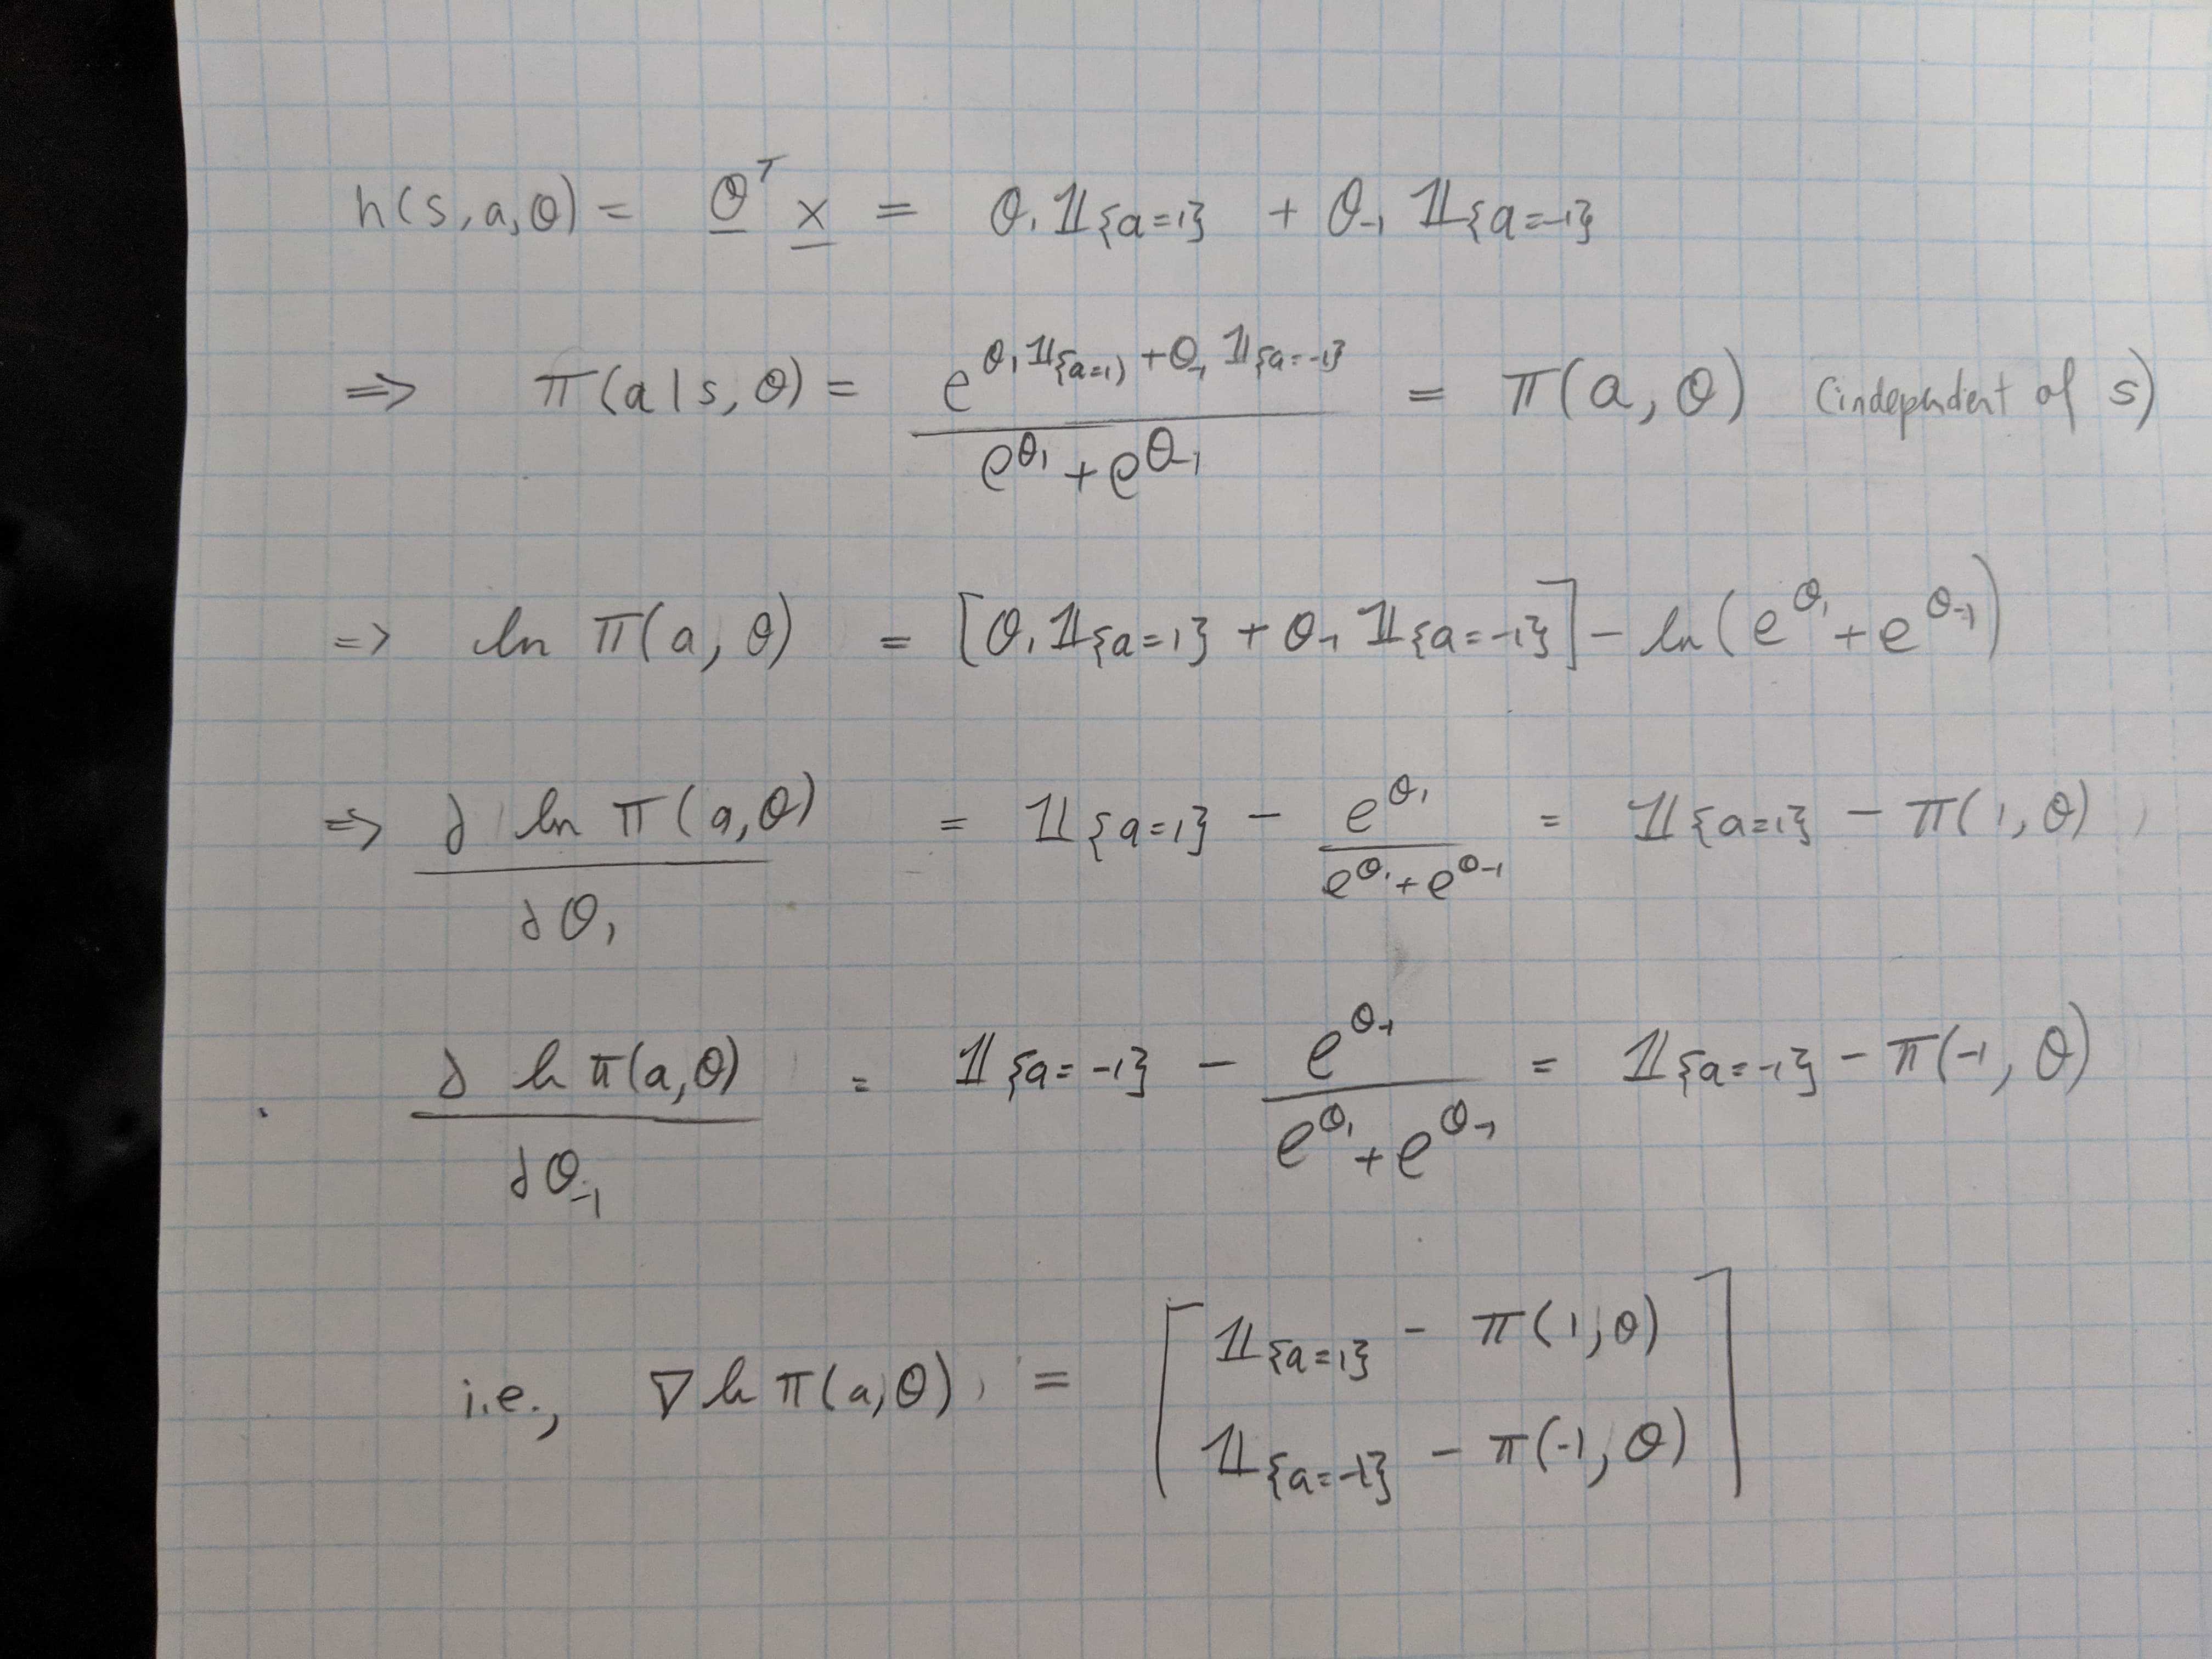
\includegraphics[width=15cm]{figures/2b.jpg}
\end{figure}

\textbf{c)} See \code{main.R} code.

\textbf{d)} The curves corresponding to step sizes $\alpha_{\theta} = 2^{-13} \text{and}
\; 2^{-14}$, (red and green curves respectively), are very similar to those presented
in the textbook. However, our return curve for step size $\alpha_{\theta} = 2^{-12}$ (blue curve) is not reflective of the one in the textbook.

\begin{figure}[H]
  \caption{Performance of REINFORCE on the short-corridor gridworld (Total reward on episode averaged over 100 runs)}
  \centering
  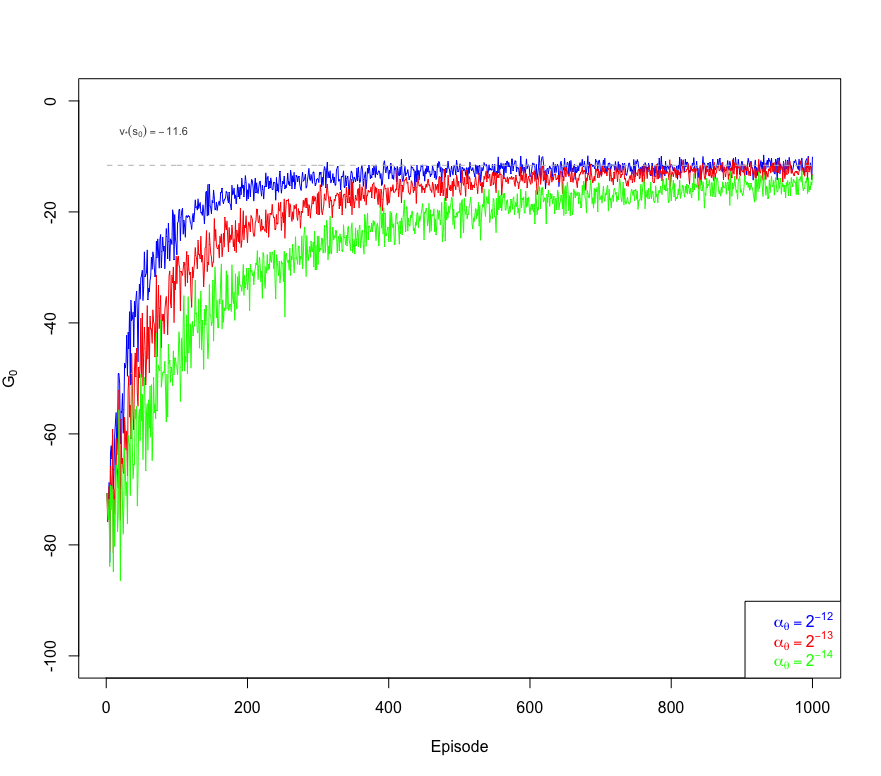
\includegraphics[width=12cm]{figures/2d1.png}
\end{figure}

\begin{figure}[H]
  \caption{Performance of REINFORCE on the short-corridor gridworld (Probability of selecting "Right" compared to the optimal probability)}
  \centering
  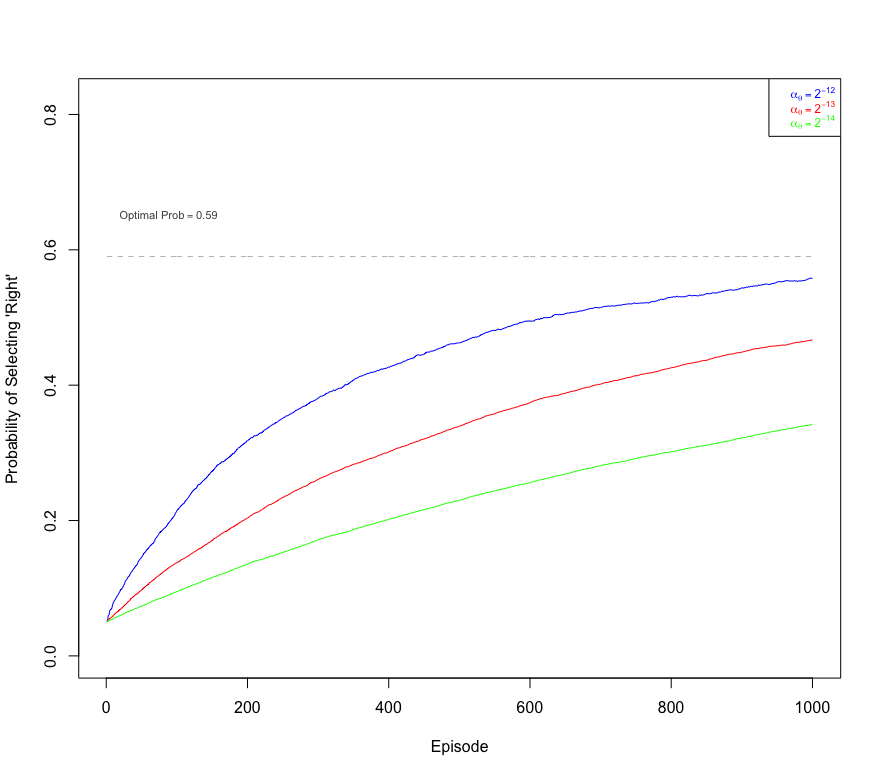
\includegraphics[width=12cm]{figures/2d2.png}
\end{figure}

\newpage

\textbf{e)} See \code{main.R} code.

\textbf{f)} The curve corresponding to step size $\alpha_{\theta} = 2^{-9}$, (green) curve is very similar to the one presented in the textbook. Regarding the red curve, the one presented in the textbook is of step size $\alpha_{\theta} = 2^{-13}$ without baseline, whereas ours is of step size $\alpha_{\theta} = 2^{-12}$ without baseline, therefore there is a discrepancy between the two red curves. However, for $\alpha_{\theta} = 2^{-12}$ the results are similar with and without baseline (red and blue). 

\begin{figure}[H]
  \caption{Performance of REINFORCE with Baseline on the short-corridor gridworld (Total reward on episode averaged over 100 runs)}
  \centering
  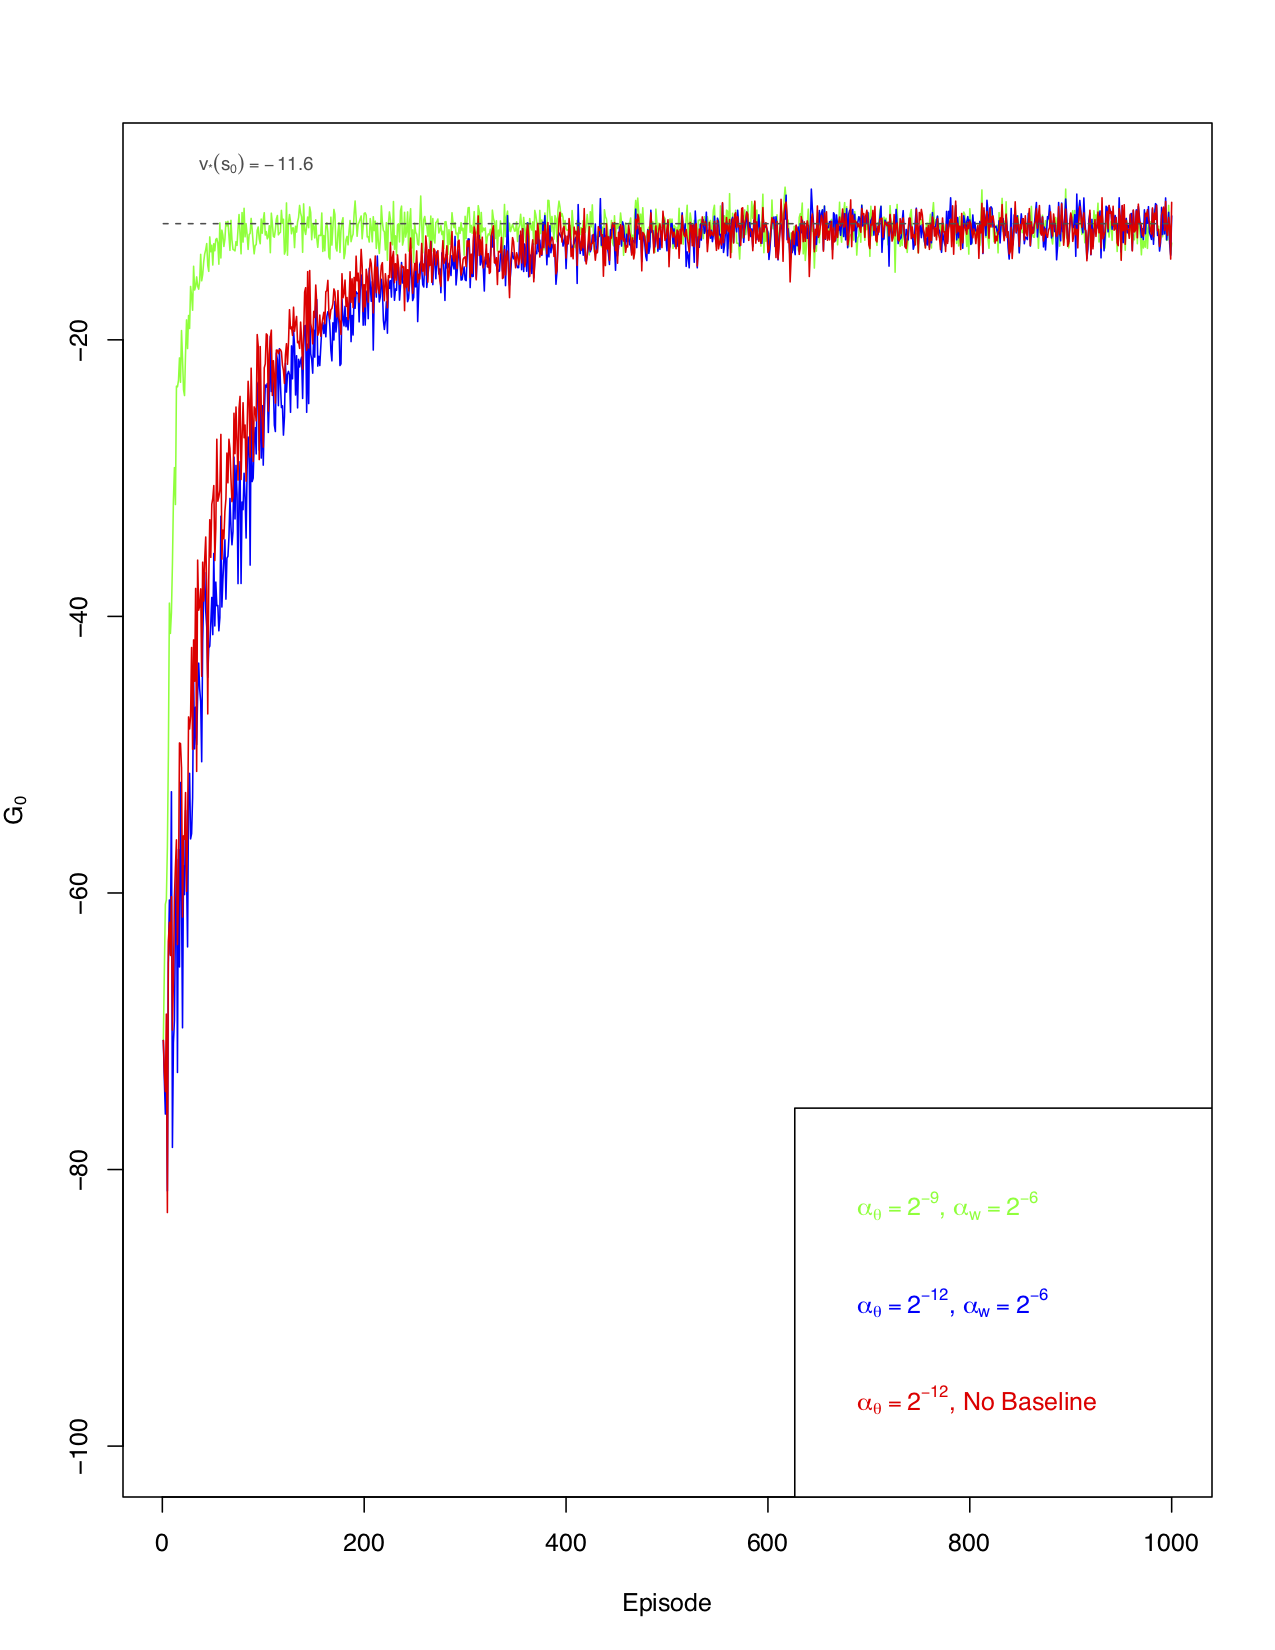
\includegraphics[width=15cm]{figures/2f.png}
\end{figure}

\end{document}
